\section{Experiments}

\subsection{Datasets}

\subsubsection{Experimental datasets}

To our knowledge, there's no existing large scale database of annotated X-ray
single particle images categorized by biological/chemical samples.  The Coherent
X-ray Data Bank (CXIDB) serves as ``a permanent public repository of data from
coherent X-ray sources" \cite{maiaCoherentXrayImaging2012}.  Table \ref{tb: SPI
experiments} is a list of all SPI experiments documented on CXIDB.  We decide to
use the raw data collected in experiment amo06516
\cite{liDiffractionDataAerosolized2020}, part of which are also available by
checking out CXIDB ID 156.  One major difference between raw data and deposited
data is that raw data contain a considerable amount of \textit{non-sample-hit}
images, which are important for real-time SPI classification tasks.  For data
labelling, we created a GUI tool (\url{https:
//github.com/carbonscott/hit-labeler}) that can label hits from multiple sources,
including raw data through \textit{psana} \cite{damianiLinacCoherentLight2016}
and HDF5 files from CXIDB.  In total, we labelled {\color{red}xxx}
\textit{single-hit}, xxx \textit{multi-hit} and xxx \textit{non-sample-hit}.  

\begin{table}
    \caption{All SPI experiments documented on CXIDB.}
    \label{tb: SPI experiments}
    %% \renewcommand{\arraystretch}{1.2}
    %% \resizebox{1.0\textwidth}{!}{
        \begin{tabularx}{\textwidth}{ l l X }
            CXIDB ID & Light Source & Sample \\
            \hline
            1        & LCLS         & Mimivirus                                                       \\
            2        & LCLS         & Mimivirus                                                       \\
            3        & FLASH        & FIB etched 20-nm-thick silicon nitride membrane                 \\
            4-8      & ALS          & Gold labeled frozen dried Saccharomyces cerevisiae yeast cells  \\
            9        & FLASH        & Iron Oxide Ellipsoids                                           \\
            10       & LCLS         & Nanorice                                                        \\
            11       & LCLS         & Magnetosomes                                                    \\
            12       & LCLS         & Tobacco mosaic virus                                            \\
            13       & LCLS         & T4 bacteriophage                                                \\
            14       & LCLS         & Paramecium bursaria Chlorella virus                             \\
            19       & LCLS         & Airborne Particulate Matter (Soot)                              \\
            20       & LCLS         & Clusters of Polystyrene Spheres                                 \\
            25       & LCLS         & Carboxysomes                                                    \\
            26       & LCLS         & Cyanobium gracile                                               \\
            27       & LCLS         & Synechococcus elongatus                                         \\
            28       & ALS          & 50 nm colloidal gold particles                                  \\
            30       & LCLS         & Mimivirus                                                       \\
            36       & LCLS         & Rice Dwarf Virus                                                \\
            37       & LCLS         & Cyanobium gracile and Synechococcus elongtatus                  \\
            56       & LCLS         & Omono River Virus                                               \\
            57       & LCLS         & Gold core and palladium shell nanoparticles                     \\
            58       & LCLS         & Coliphage PR772                                                 \\
            78       & LCLS         & RNA polymerase II                                               \\
            84       & ESRF         & Gold structure (largest diameter about 1.1 um)                  \\
            88       & LCLS         & PR772                                                           \\
            119      & LCLS         & Sucrose                                                         \\
            146      & FLASH        & Xenon nanoclusters                                              \\
            155      & LCLS         & Melbournevirus                                                  \\
            156      & LCLS         & Coliphage PR772                                                 \\
        \end{tabularx}
    %% }
\end{table}


\subsubsection{Simulated datasets}

There's no existing large scale database of annotated SPI images generated by
physics-based simulation.  To investigate generalizability of our SPI classifier,
it's essential to have a large dataset of simulated SPI images. We resort to
\textit{skopi} \cite{peckSkopiSimulationPackage2021}, a GPU-based program for
simulating diffractive images from noncrystalline biomolecules, for concurrently
simulating high-resolution SPI scattering and providing accurate labels in an
automated manner at scale.  Our primary interest is to explore the model
generalizability on \textit{large} single particles, considering the
state-of-art resolution ever reached in an SPI experiment is still at the
nanometer level ($>$ 10 $nm$) {\color{red} (need to fact-check)} unlike in
protein crystallography that studies biological structures at the angstrom
level.  PDB statistics offers direct insights into PDB data distribution by
molecular weight (\url{https:
//www.rcsb.org/stats/distribution-molecular-weight-structure}).  We focus on
\textit{large} particles with molecular weights over 380 $KDa$.  Fig. \ref{fig:
num atom per bio assem} describes the population frequency of the atom numbers
per biological assembly with each area representing 50 PDB items.  The atom
numbers spread across three orders of magnitudes ($10^4\text{-}10^6$).  96.0\%
of \textit{large} particles have $10^4$ atoms, and only 1.2\% have massive
$10^6$ atom numbers. Simulated datasets are generated by setting the detector
distance at 100.0 $mm$ and photon energy at 1.660 $keV$.  Random rotation is
also applied as a means of data augmentation.  

\begin{figure}
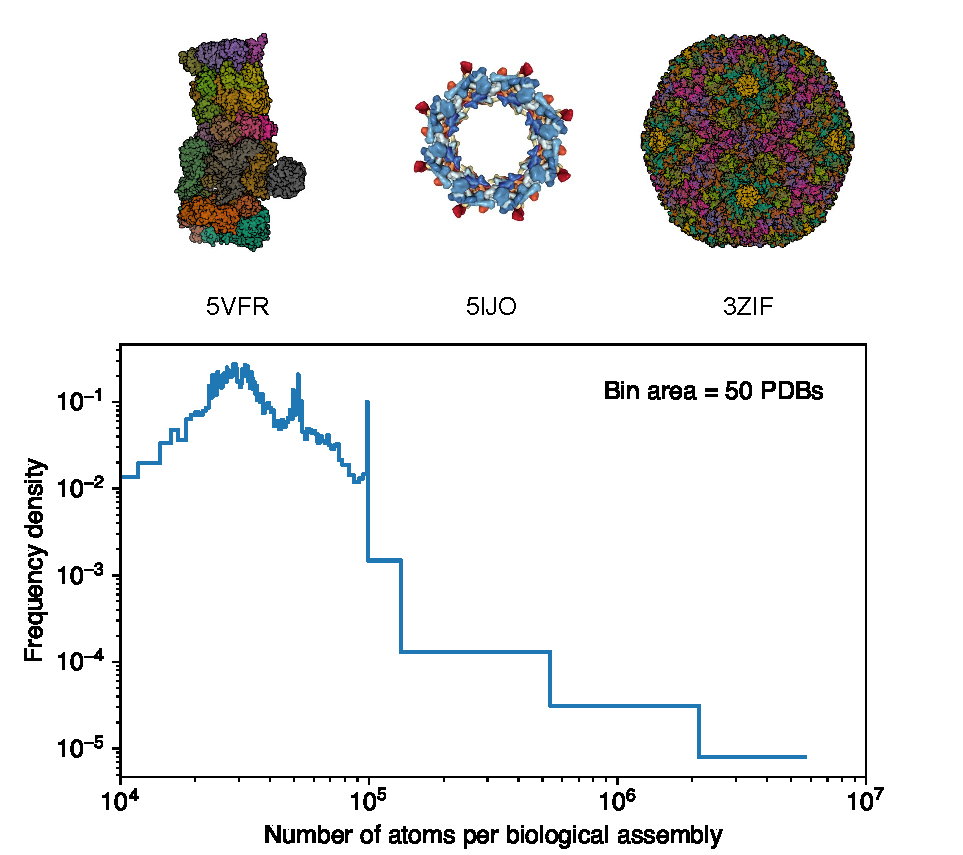
\includegraphics[width=1.0\textwidth,keepaspectratio]
{./figures/num_atom_per_bio_assem.pdf}
\caption{Number of atom per biological assembly. {\color{red} Need to indicate where
those molecular graphs are from.}}
\label{fig: num atom per bio assem}
\end{figure}


\subsection{Effects of data variety on model performance}

We split our experimental dataset into training set, validation set and test
set.  This is a standard practice that evaluates the goodness of a model on a
given dataset.  Data split can be tricky to handle when the size of a given
dataset is small, which is one of the challenges we will face in training a
real-time classifier during data collection.  On the other hand, data
augmentation can effortlessly increase the volume of the dataset, but can our
model achieve infinitely better performance with data augmentation?  The short
answer is `NO', and we will discuss how the varieties of uniquely `looking' data
impact model performance.  We point out that when a flat detector is used and
aligned perpendicularly to the beam path, any rotation of a diffraction image
along this beam path doesn't add a new variety to the dataset for model
training.  For example, if a training dataset only consists of images generated
by randomly rotating a reference image along the beam path, our model can
successfully identify the labels of those augmented images, but it will likely
fail to recognize images with other unique patterns.  We consider that every
manually labelled image looks uniquely as the chance of labelling two images
differed by a matter of rotation is very little.  In Table \ref{tb : metadata}
and \ref{tb : performance}, we provide metadata and confusion matrices,
respectively, of four distinct experiments to demonstrate the effects of data
variety on model performance.  

We use the same data spliting strategy in experiment 1 and 2, which is 25.0\%
/37.5\%/73.5\% (train/validate/test) as seen in Table \ref{tb : metadata}.  We
sample 40 unique images per class, but there are only 18 \textit{non-sample-hit}
in the training set.  We apply random rotations along the beam path to the
sampled images, and the total number of images amounts to 2000 for the training
set and the validation set, respectively.  In experiment 2, similar random
rotations result in 4000 images in the training set and the validation set,
respectively.  Despite having double the number of images in training,
experiment 2 shows a slightly worse performance, especially in the recall of
predicting \textit{multi-hit} according to Table \ref{tb : performance} .  Since
recall measures the percentage of images correctly predicted for a class, it
implies that the model performance can't be improved through more data
augmentation.  We hypothesize that the data variety is still too low when only
25.0\% is assigned to the training set.  

We choose a new data spliting strategy in experiment 3 and 4, which is 50.0\%
/25.0\%/25.0\% (train/validate/test) as depicted in Table \ref{tb : metadata}.
In experiment 3, we still sample 40 images per class despite having more
candidates to choose thanks to the 50.0\% data split for training.  Again, we
apply similar random rotations to the sampled images, and the total number of
images is 2000 for training and validation, respectively.  As shown in Table
\ref{tb : performance}, the model in experiment 3 still can't improve its recall
of 90\% in predicting \textit{multi-hit}.  It seems to signal that 40 images per
class is not large enough to cover the data distribution in the training set.
Then, we decide to sample 80 images per class in experiment 4, despite only 44
\textit{non-sample-hit} are avaiable in the training set.  A total of 2000
images for training and validation, respectively, are arranged through the same
random rotation technique.  In Table \ref{tb : performance}, the recall of
predicting \textit{multi-hit} in experiment 4 increases to 97\%, a substantial
improvement in constrast to $\sim 90\%$ in all previous three experiments.  

To sum it up, data variety plays a critical role in dictating the model
performance by covering the space where data are distributed.  From a practical
perspective, a good precision of predicting \textit{single-hit} would suffice
for our use that is to keep only \textit{single-hit}.  However, it is recall
that indicates whether the data variety is sufficient, which is the underlying
limiting factor that prevents model from achieving a better precision.  



%% Two data spliting
%% strategy are used in the four experiments:  split in experiment 1 and 2; 50.5\%/25.0\%/25.0\% split in
%% experiment 3 and 4.  Obviously, experiment 3 and 4 have larger variety of
%% uniquely `looking' data in the training set.  Experiment 1 and 2 have exactly
%% the same unique images per class, but experiment 2 has a larger data volume as
%% more images are generated by data augmentation.  in Table \ref{tb : performance}, 


\begin{table}

    \caption{
        The metadata of four experiments that are used to illustrate the
        limiting factors of model performance from the training data standpoint.  \#
        denotes `number of images'.  The numbers in the `Unique \# $/$ class' column
        follow the order of \textit{non-sample-hit}, \textit{single-hit} and
        \textit{multi-hit}.  \# (Train) and \# (Validation) are the number of images,
        including those generated from data augmentation, used in model training and
        validation, respectively.  The last column tells the fraction of all
        labelled images used in the training set.  
    }
    \label{tb : metadata}
    %% \renewcommand{\arraystretch}{1.2}

    %% \centering
    %% \resizebox{1.0\textwidth}{!}{
        \begin{tabularx}{\linewdith}{ l c c c c }
            Experiment &   $\dfrac{Unique \#}{class}$  &  \# (Train) & \# (Validation) & $\dfrac{\text{\#Training}}{\text{\#Total}}$ \\
            \hline
            1          &   18,40,40             &  2000       & 2000            & 0.25      \\
            2          &   18,40,40             &  4000       & 4000            & 0.25      \\
            3          &   40,40,40             &  2000       & 2000            & 0.50      \\
            4          &   44,80,80             &  2000       & 2000            & 0.50      \\
        \end{tabularx}
    %% }
\end{table}



\begin{table}
    \caption{
        Confusion matrix for each experiment mentioned in Table. \ref{tb :
        metadata}.
    }

    \label{tb : performance}

    %% \centering
    %% \renewcommand{\arraystretch}{1.2}
    %% \resizebox{1.0\columnwidth}{!}{
        \begin{tabularx}{\linewidth}{ l | X X X X X X X X }
            \textbf{Experiment 1} &  N(A) & S(A) & M(A) & ACC  & PRE  & REC           & SPE  & F1   \\
            \hline
            N(P)                  &  335  & 0    & 10   & 0.99 & 0.97 & 1.00          & 0.98 & 0.99 \\
            S(P)                  &  0    & 333  & 24   & 0.97 & 0.93 & 0.99          & 0.96 & 0.96 \\
            M(P)                  &  0    & 5    & 293  & 0.96 & 0.98 & \textbf{0.90} & 0.99 & 0.94 \\
            \hline
            \textbf{Experiment 2} &  N(A) & S(A)  & M(A) & ACC  & PRE  & REC           & SPE  & F1   \\
            \hline
            N(P)                  &  335  & 1     & 9    & 0.99 & 0.97 & 1.00          & 0.98 & 0.99 \\
            S(P)                  &  0    & 327   & 28   & 0.96 & 0.92 & 0.97          & 0.97 & 0.94 \\
            M(P)                  &  0    & 10    & 290  & 0.95 & 0.97 & \textbf{0.89} & 0.99 & 0.93 \\
            \hline
            \textbf{Experiment 3} &  N(A) & S(A)   & M(A) & ACC  & PRE  & REC           & SPE  & F1   \\
            \hline
            N(P)                  &  331  & 0      & 13   & 0.99 & 0.96 & 1.00          & 0.98 & 0.98 \\
            S(P)                  &  0    & 339    & 19   & 0.97 & 0.95 & 0.98          & 0.97 & 0.96 \\
            M(P)                  &  0    & 6      & 292  & 0.96 & 0.98 & \textbf{0.90} & 0.99 & 0.94 \\
            \hline
            \textbf{Experiment 4} &  N(A) & S(A)   & M(A) & ACC  & PRE  & REC           & SPE  & F1   \\
            \hline
            N(P)                  &  331  & 1      & 7    & 0.99 & 0.98 & 1.00          & 0.99 & 0.99 \\
            S(P)                  &  0    & 340    & 4    & 0.99 & 0.99 & 0.99          & 0.99 & 0.99 \\
            M(P)                  &  0    & 4      & 313  & 0.98 & 0.99 & \textbf{0.97} & 0.99 & 0.98 \\
        \end{tabularx}
    %% }
\end{table}
